\documentclass[tikz]{standalone}
\usetikzlibrary{decorations.pathreplacing}

\begin{document}
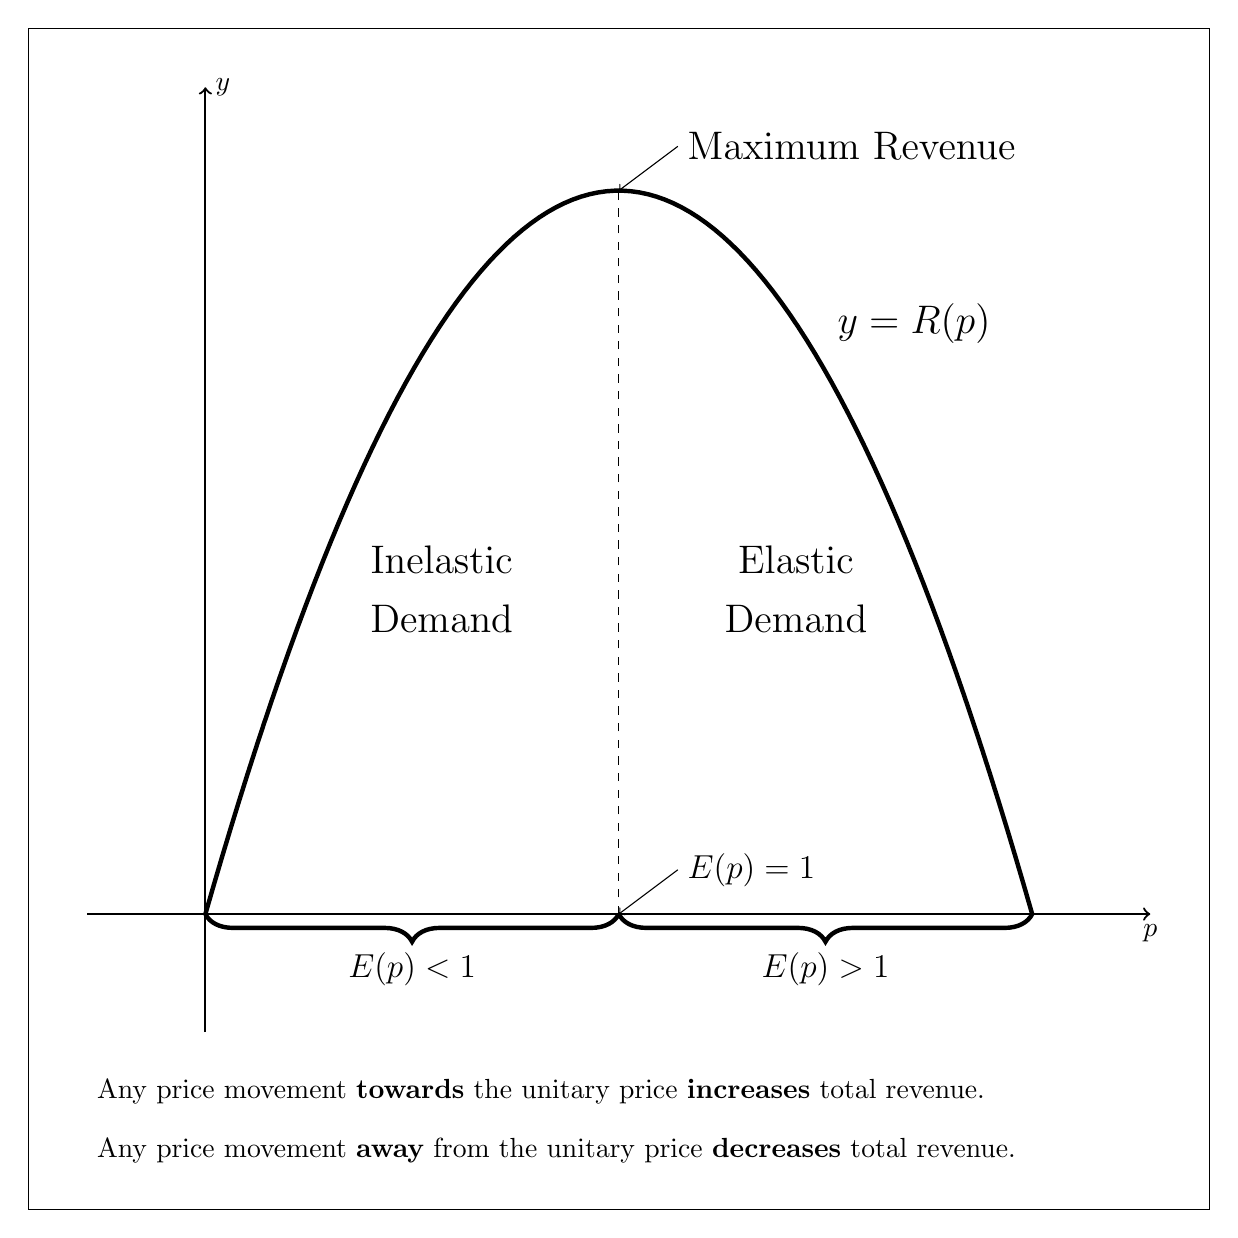
\begin{tikzpicture}[scale=1.5]

% create a white background, with a black frame
\draw [fill=white] (-1.5,-2.5) rectangle (8.5,7.5);  % black border

% define point of tangency and second point on the curve
\coordinate (pointA) at (1,1.4);   
\coordinate (pointB) at (4,3.8416); 

% draw axes
\draw[->,thick] (-1,0) -- (8,0) node[below] {$p$}; 
\draw[->,thick] (0,-1) -- (0,7) node[right] {$y$};

% plot function
\draw[ultra thick,variable=\x] plot [domain=0:7,samples=100] (\x,{(7*\x - \x*\x)/2});
\node at (6,5) {\Large $y = R(p)$};

% \plot dashed lin
\draw[dashed] (3.5,0) -- (3.5,6.125);
%% plot tangent line
%\draw[ultra thick,variable=\x,blue]
%plot [domain=-1:5] (\x,{0.471 * (\x - 1) + 1.4}) node[right] {tangent line};
%% plot secant line
%\draw[ultra thick,variable=\x,red]
%plot [domain=-1:5] (\x,{0.815*(\x - 1) + 1.4}) node[right] {secant line};

%% dashed lines and corresponding labels
%\draw[dashed] (0,1.4) node[left] {$f(a)$} -| (1,0) node[below] {$a$};
%\draw[dashed] (0,3.8416) node[left] {$f(a+h)$} -| (4,0) node[below] {$a+h$};

%% draw points
%\fill[black] (pointA) circle (2pt);
%\fill[red] (pointB) circle (2pt);

% E(p) < 1
\draw [ultra thick,decorate,decoration={brace,amplitude=10pt},yshift=0pt]
(3.5,0) -- (0,0) node [black,midway,yshift=-20pt] {\large $E(p) < 1$};

% E(p) > 1
\draw [ultra thick,decorate,decoration={brace,amplitude=10pt},yshift=0pt]
(7,0) -- (3.5,0) node [black,midway,yshift=-20pt] {\large $E(p) > 1$};


\node at (2,3) {\Large Inelastic};
\node at (2,2.5) {\Large Demand};
\node at (5,3) {\Large Elastic};
\node at (5,2.5) {\Large Demand};


%% label max revenue
\draw[<-] (3.5,6.125) -- (4,6.5) node[right] {\Large Maximum Revenue};

%% label unitary point
\draw[<-] (3.5,0) -- (4,0.375) node[right] {\large $E(p) = 1$};


\node[right] at (-1,-1.5) {Any price movement {\bf towards} the unitary price {\bf increases} total revenue.};

\node[right] at (-1,-2.0) {Any price movement {\bf away} from the unitary price {\bf decreases} total revenue.};

\end{tikzpicture}
\end{document}
